\chapter{研究方法}
\label{章:研究方法}

\section{拄好長度斷詞}
\label{節:拄好長度斷詞}

\begin{table}
\caption{長詞優先毋著的情形}
\label{表:長詞優先佇一寡例有問題}
\centering
\begin{tabular}{c|c}
方法 & 結果\\
\hline
長詞優先(對後壁) & 猶 掠做 唱歌 仔 戲 真 簡單\\
答案 & 猶 掠做 唱 歌仔戲 真簡單\\
\hline
長詞優先(對後壁) & 甚至 和 國 小學生 嘛 想 袂 開\\
答案 & 甚至 和 國小 學生 嘛 想 袂 開\\
\end{tabular}
\end{table}

\begin{table}
\caption{拄好長度成本}
\label{表:拄好長度成本}
\centering
\begin{tabular}{c|c}
斷詞結果 & 拄好長度成本\\
\hline
猶 掠做 唱歌 仔 戲 真 簡單 & $…+\frac{1}{2}+\frac{1}{1}+\frac{1}{1}+…$\\
猶 掠做 唱 歌仔戲 真簡單 & $…+\frac{1}{1}+\frac{1}{3}+…$\\
\hline
甚至 和 國 小學生 嘛 想 袂 開 & $…+\frac{1}{1}+\frac{1}{3}+…$\\
甚至 和 國小 學生 嘛 想 袂 開 & $…+\frac{1}{2}+\frac{1}{2}+…$\\
\end{tabular}
\end{table}

\ref{節:閩南語斷詞}節講愛比較斷詞的方法,
定用的斷詞方法有\ref{節:長詞優先斷詞}節的長詞優先,
佇遮本論文提出一个「節:拄好長度斷詞」的方法。

%ㄍㄛˊ

因為上長詞有時陣會揀著無好的組合,
親像表\ref{表:長詞優先佇一寡例有問題},
長詞優先有的情形會斷毋著。
觀察這个情形,
第一組例是斷詞結果的詞數比答案閣加一个,
斷出來的詞傷濟矣。
第二組例是斷詞結果佮答案攏是斷詞兩个詞,
因為斷詞結果共四字攏分配做一字詞佮三字詞,
字數分配無齊勻。

綜合這兩个觀察,
本論文提出「拄好長度斷詞」。
斷詞的方法是維特比(Viterbi)算法,
成本函式是訂做一字詞1分、兩字詞1/2分、三字詞1/3分、四字詞1/4分、…。
用面頂表的例,
算出來的成本會當看表\ref{表:拄好長度成本}
%數學式

\section{未知詞另外翻譯}
\label{節:未知詞另外翻譯}

\begin{figure}
\centerline{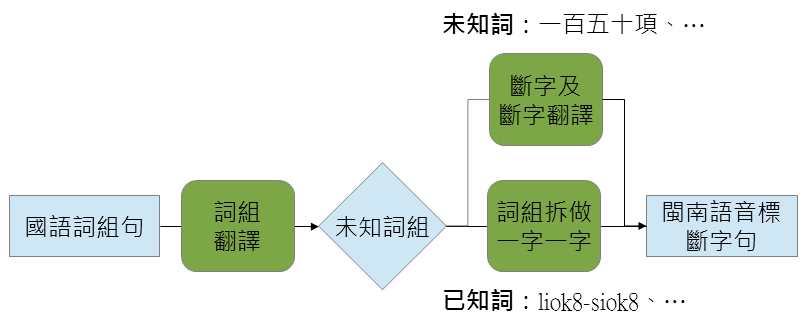
\includegraphics[keepaspectratio,width=40em]{圖/未知詞另外翻譯}}
\caption{未知詞另外翻譯流程}
\label{未知詞另外翻譯}
\end{figure}

對\ref{節:未知詞問題}節來看,
用斷詞翻譯會拄著未知詞的問題。
準若咱用斷詞的翻譯模型,
拄著未知詞的時陣,
這个未知詞會使提予斷字翻譯模型去翻譯,
就是講「陸續 開放 一百五十項 的 規費」提予斷詞組模型翻譯,
得著「liok8-siok8 khai1-hong3 一百五十項 e5 規費」,
閣來共「一百五十項」佮「規費」這兩个詞組切做斷字「一 百 五 十 項」佮「規 費」,
閣擲去斷字模型翻譯,流程會當看圖\ref{未知詞另外翻譯}。

\section{漢羅全羅對齊}
\label{節:漢羅全羅對齊}
佇\ref{節:數位典藏}節有講著,數位典藏是提供漢羅佮全羅的對照,因為咱的翻譯需要一个漢字對一个音標的一對一,所以愛共數位典藏伊原本一段對齊一段的語料改做一字對一字。
而且愛注意數位典藏佇2006年完成,教育部的漢字規範對2007年才公佈,所以⿰因兩个的用字規範嘛是無仝款的。
毋過數位典藏的語料倩人整理的時陣內部有訂標準,伊的漢字有一半以上攏是會用得的。
本論文以教育部的為主,
對齊的做法是共全羅逐字攏去對看覓漢羅,
看佗一个組合會佇字典內底,
揣出上長的組合。

%有1個少年人;伊抵tng7 teh 想
%U7 chit8 e5 siau3-lian5 lang5; i tu2-tng7 teh siuN7 phok-su7 lun7-bun5, 

\section{補全漢佮全羅}
\label{節:補全漢佮全羅}
佇\ref{節:整理語料}節有講著,
閩南語的完整資訊有全漢、全羅、斷詞三个,
若全部的語料攏有這三種資訊,
翻譯效果會閣較好。

斷詞的部份佇\ref{節:拄好長度斷詞}節有討論矣,
這節的重點是下佇按怎自動整理語料的全漢佮全羅,
替\ji{⿰因}補起哩欠的漢字佮羅馬音標。

因為有的詞可能一字音標、一字是漢字,
親像「彰化」,寫做「tsiong1化」。
本論文提出一个做法,
整理語料的時猶原用斷詞方法,
毋過用的辭典愛小可仔改變,
逐个詞的全部形式攏愛加佇辭典內底,
閣愛加「彰hua3」、「彰tsiong1 hua3」、
…攏總九種\footnote{一个字的資訊可能是「漢字」、「音標」、「漢字音標攏有」三種其中一種。
兩字,攏總$3^{2}=9$種}。

%為著查字典的速度閣較緊,
%就親像圖XX仝款,
%逐个詞一字一字處理落來,
%逐字分做漢字、音標、一對一三个點,
%第二个字閣佇這三个點閣生落去,
%毋過第一个字有佮別的詞仝款,
%就會使公家一个點,
%親像「彰化」「將來」「將軍庄」,
%因為限制上長四字詞\footnote{照教育部的「臺灣閩南語羅馬字拼音方案連字符使用原則」,
%有可能有五字詞,毋過這擺實驗限制四字詞},
%一个詞上濟產生120點\footnote{第一層加到第四層,$3^{1}+3^{2}+3^{3}+3^{4}=120$},
%毋過揣候選詞的時間複雜度是$O(1)$。

決定斷詞斷佇佗位了後,
逐个斷詞的所在可能有超過一个的候選詞,
%「彰化的米誠好食」,
上尾閣用語言模型,
配合維特比算法,
揀出機率上懸的語句。


\section{語言分類特徵}
\label{節:語言分類特徵}

\ref{節:語言分類}節有講,
閩南語佮華語的以字為單位的語言模型效果無好,
為著予電腦會當分別閩南語佮華語,
咱就愛準備幾項閩南語佮華語無仝的特徵。
本論文提出一个以斷詞資訊做判斷特徵的方法,
除了以斷詞算語言模型以外,
閣加入斷詞了一字詞、兩字詞、三字詞、四字詞的詞數。

毋過按呢閣無夠
閩南語佮華語上大差別就是用詞無仝,
閩南語寫「食飯」、「無法度」,
華語寫「吃飯」、「沒辦法」,
所以咱揀定用詞出來,
當作咱的特徵之一。

毋過閩南語佮華語有誠濟共同詞,
親像「火車」、「電腦」,
\ji{⿰因}寫法是仝款的,
咱袂使直接提定用詞來做,
因為內底會有共同詞,
所以咱愛揀出無共同詞的「特徵詞」。

選特徵詞的方法是先統計閩南語語料佮華語語料,
分別揣出n个定用詞\footnote{有算標點符號},
了後揀出頭前m个閩南語定用詞,
而且這m个閩南語定用詞無出現佇華語n个定用詞,
這m个詞阮就號做閩南語特徵詞。
華語部份嘛仝款,
揀出頭前m个華語定用詞,
這m个詞袂使出現佇閩南語的n个定用詞,
這m个詞就是華語的特徵詞。

%看圖
%加例


\begin{figure}
\centerline{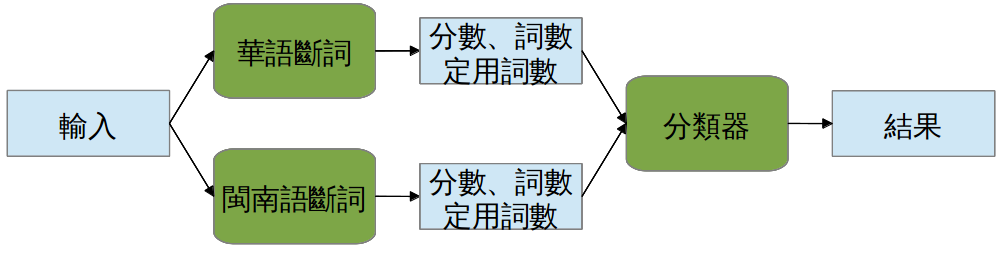
\includegraphics[keepaspectratio,width=40em]{圖/判斷語言架構}}
\caption{判斷語言流程}
\label{圖:判斷語言架構}
\end{figure}






